\subsubsection{KD-træer}
\label{sec:kdtree}

Et K-dimensionelt træ (KD-træ), er en abstrakt datastruktur som bl.a.\ andvendes til opdeling af 'rum'. Et KD-træ er repræsenteret som et binært træ, dvs.\ at
hver gren i træet har yderligere to grene indtil bladene nåes (se figur ...) herunder. 

\begin{figure}[H]
  \centering
  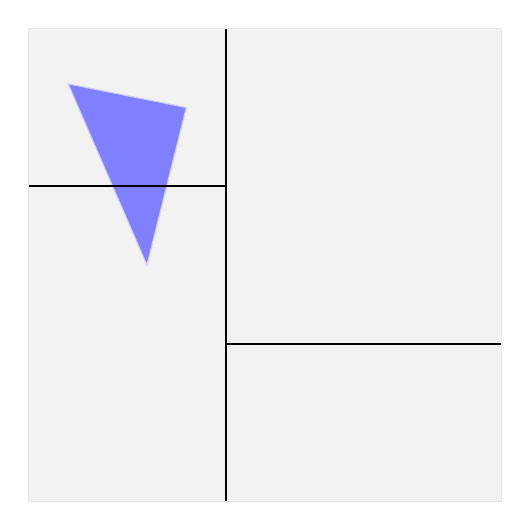
\begin{tikzpicture}
    \path[fill=gray!10, draw=gray!20] (3,3) -- (3,-3) -- (-3,-3) -- (-3,3) -- (3,3);
    
    \path[fill=blue!50, draw=blue!20] (-1,2) -- (-2.5,2.3) -- (-1.5,0) -- (-1,2);
    
    \draw [black, thick] (-0.5, -3) -- (-0.5, 3);
    \draw [black, thick] (-0.5, -1) -- ( 3,  -1);
    \draw [black, thick] (-0.5,  1) -- (-3,   1);
    % triangle
    % \draw [blue!50, thick, -{Stealth[width=3mm, length=3mm]}] (2,-4,3) -- (3,-4,1);
    % \draw [blue!50, thick, -{Stealth[width=3mm, length=3mm]}] (2,-4,3) -- (1,-4,2);
    % \draw [blue!50, thick, -{Stealth[width=3mm, length=3mm]}] (2,-4,3) -- (2,-2,3);
    % \draw [black,   thick, -{Stealth[width=2mm, length=2mm]}] (2,-4,3) -- (2,-4,2);
    % \node [above] at (2,-3,3) {$\vv{n}$};
    % \node [above] at (2,-4,3) {$A$};
    % \draw plot [mark=*, mark size=1] coordinates{(2,-4,3) }; 
    % \node [left] at (3,-4,1) {$B$};
    % \draw plot [mark=*, mark size=1] coordinates{(3,-4,1) }; 
    % \node [below] at (1,-4,2) {$C$};
    % \draw plot [mark=*, mark size=1] coordinates{(1,-4,2) };
    
    % ray
    % \node [above right] at (0,0,0) {$P_0$};
    % \draw plot [mark=*, mark size=1] coordinates{(0,0,0) };
    % \node [above right] at (0.25,-0.5,0.25) {$\vv{r}$};
    % \draw [black, thick] (0,0,0) -- (2,-4,2);
    % \draw [blue!50, thick, |-|] (0.1,0,-0.1) -- (2.1,-4,1.9);
    % \node [below left] at (1,-2,1) {$t_A$};
    % \node [black, above left] at (2.5,-4,2) {$P(t_A)$};
    % \draw [black, thick, -{Stealth[width=3mm, length=3mm]}] (0,0,0) -- (0.5,-1,0.5);
    % \draw plot [mark=*, mark size=1] coordinates{(2,-4,2) };
  \end{tikzpicture}
  \caption{KD-træ}
  \label{fig:kd-tree}
\end{figure}

Med et KD-træ opdeles et rum efter værdier, højere eller lavere end et taktisk udvalgt delingspunkt (se figur ...),
således at alle værdier i en gren, enten er højere eller lavere end den gren de udspringer fra. Denne  opdeling fortsætter indtil værdierne i en gren er trivielle at behandle, herved kaldes en sådan gren for et blad.
